\subsection{Custo das Aberturas vistas por $r \in T_c$}

Somente o peso do custo das aberturas do gol vistas pelos robôs do time foi
alterado para $1000$. Os resultados no planejamento são apresentados na
Figura~\ref{fig:see_enemy_goal_1000}. Fica evidente em ambos os ambientes de
ataque e defesa que os robôs se posicionaram o mais próximo possível do gol de
$T_{ad}$, se limitando apenas pela penalização por proximidade do gol
adversário.

\begin{figure}[H]
  \centering
  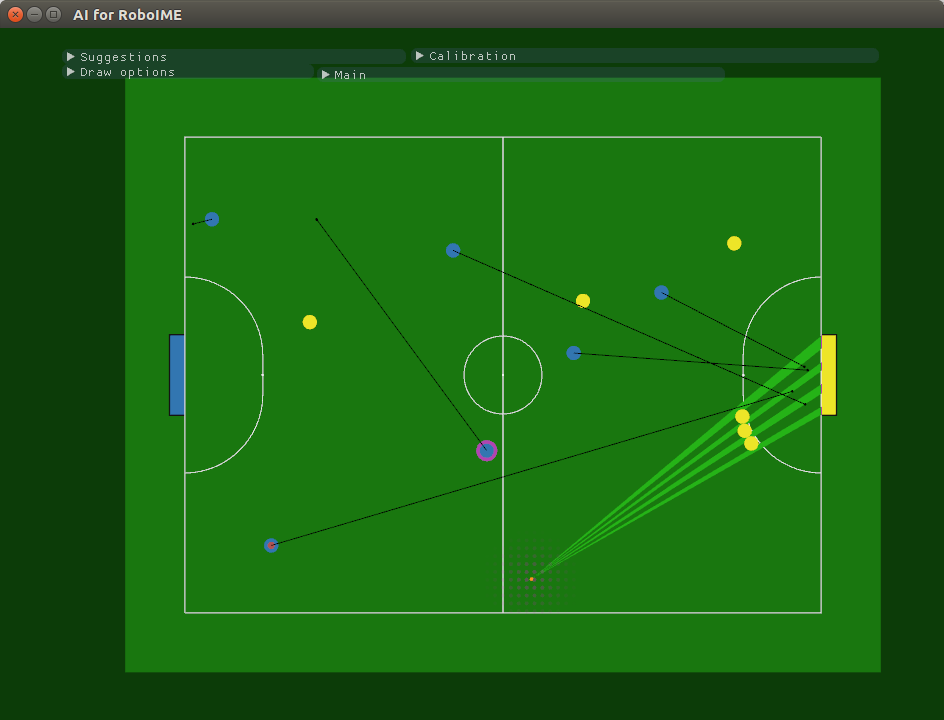
\includegraphics[width= 0.8\linewidth]{result/see_enemy_goal_atq_1000}
  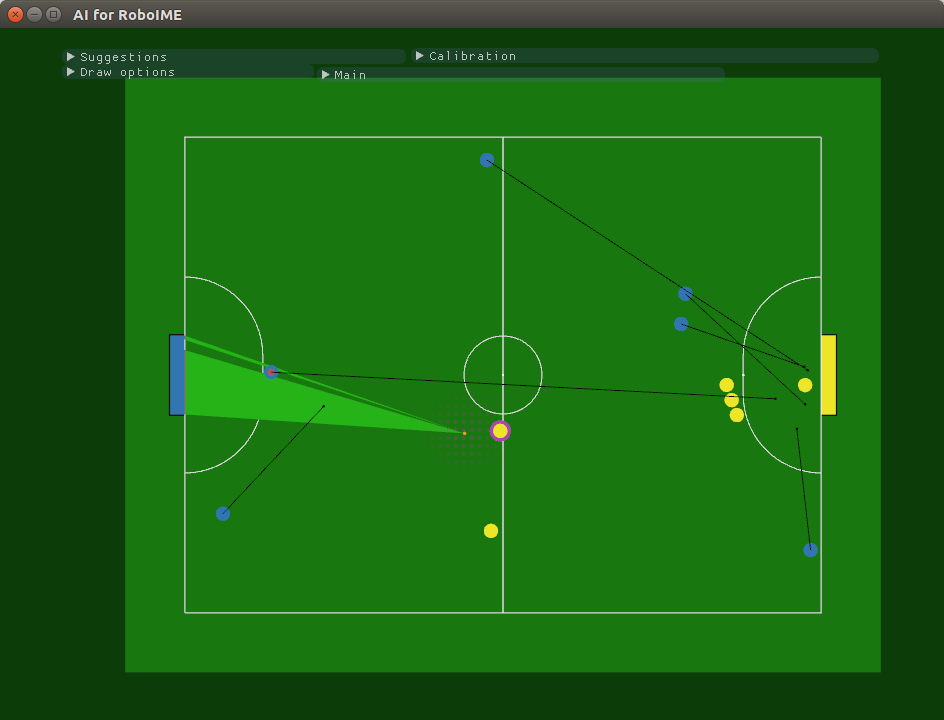
\includegraphics[width= 0.8\linewidth]{result/see_enemy_goal_def_1000}
  \caption{Planejamento com os parâmetros iniciais e com o peso do custo das
  aberturas do gol vistas pelos robôs do time igual a $1000$.  No ataque (acima)
  e na defesa (abaixo)}\label{fig:see_enemy_goal_1000}
\end{figure}

% vim: tw=80 et ts=2 sw=2 sts=2 ft=tex
